\indent \section{Проектирование интерфейса парсера русского языка к онтологии}

В данной главе  рассмотрено внешнее и внутреннее проектирование. Внешнее проектирование --- этап проектирования объекта как сложной иерархической системы, состоящий в рассмотрении его как части системы более высокого уровня. Результатом такого проектирования является исходный вариант технического задания, которое может уточняться и корректироваться в процессе внутреннего проектирования объекта. Внутреннее проектирование - этап проектирования объекта как сложной иерархической системы, выполняемый на основании внешнего проектирования и состоящий в рассмотрении его как самостоятельной системы.

\subsection{Внешнее проектирование}

\subsubsection{Целеполагание}

Задача системы --- взять на себя взаимодействие с хранилищами синтаксической информации, заменив локальные словари парсеров, таким образом достигнув \textbf{глобальную цель} --- повышение качества используемых парсерами данных о синтаксисе ЕЯ.

Глобальную цель можно представить в виде композиции следующих локальных целей:

\begin{list}{\labelitemi}{\leftmargin=1.5cm}
	\item обеспечить взаимодействие синтаксического парсера с модулем на уровне API;
	\item обеспечить генерацию SPARQL-запросов из получаемых парсером слов;
	\item обеспечить сетевое взаимодействие с внешним хранилищем синтаксических знаний (OWL, RDF Scheme);
	\item обеспечить преобразование полученного в формате онтологии ответа в правила парсера и передачу их в парсер.
\end{list}

Достижение вышеупомянутых целей позволит снять с разработчика парсера ответственность за разработку и поддержание грамматики парсера, позволит использовать в работе парсера наиболее полный и корректный источник знаний, упростит разработку и развитие парсера.

\subsubsection{Выработка требований к системе}

Поскольку модуль взаимодействия парсера русского языка с онтологией (далее Модуль) представляет собой интерфейс, наиболее критичным при проектировании являются протоколы и способы обмена информацией в точках соприкосновения Модуля с соединяемыми элементами надсистемы.

При внешнем проектировании в данной работе в качестве экземпляра парсера используется реализация парсера грамматики связей от AbiWord \cite{abiparser}. По состоянию на май 2013, он находится в версии 4.7 и предоставляет готовую грамматику для русского языка, которую можно использовать в качестве образца для генерации правил и для контроля корректности работы Модуля.

Упомянутый парсер предоставляет API \cite{api}, с помощью которого разумно реализовать взаимодействие с Модулем. Такая реализация значительно увеличит производительность результирующего решения за счёт отсутствия каналов передачи информации между парсером и Модулем и нивелирования накладных расходов на двустороннее преобразование типов данных в точке соприкосновения. С другой стороны, реализация на основе API неизбежно накладывает ограничения на язык программирования: у выбранной технологиии должна быть возможность реализовать бинарный интерфейс с программами, написанными на C.

Со стороны онтологии Модуль должен использовать технологию, предоставляемую стэком Semantic Web (рисунок \ref{fig:swstack}). Жёлтым цветом на рисунке выделены протоколы, используемые для взаимодействия с семантическими хранилищами извне (язык запросов SPARQL и формат описания RDF). 

\begin{figure}[H]
	\centering
		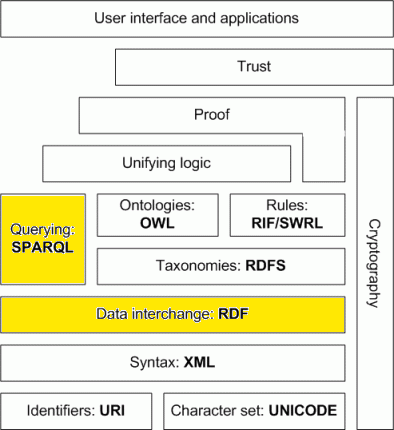
\includegraphics[scale=1.0]{images/swstack.png}
	\caption{\small Стэк технологий SW}
	\label{fig:swstack}
\end{figure} 

Таким образом, со стороны семантического хранилища Модуль должен реализовывать обмен данными посредством сетевого протокола HTTP, отправляемые данные имеют формат запроса SPARQL, принимаемые --- RDF (XML). Полученный от хранилища XML необходимо десериализовать (преобразовать во внутренний формат данных) и передать парсеру извлечённые из него данные.

В демонстрационных целях, в качестве хранилища будет использовать самостоятельно созданная OWL-онтология.

Поскольку проектируемый Модуль базируется на разработке AbiWord, являющейся открытым проектом и распространяющейся под лицензией GPL \cite{gpl}, код Модуля также обязан подчиняться правилам лицензии, быть открытым и свободно распространяемым. 

\subsubsection{Выработка требований к функционированию}

Второй ключевой характеристикой функционирования является скорость одной итерации от получения слова до возвращения правил парсеру. Синтаксическая информация изменяется крайне редко (в основном, в случае корректировок и дополнений), поэтому вероятность изменения полученных правил за время их оборота в системе пренебрежимо мала. С этой точки зрения, разумно обязать Модуль кэшировать информацию по уже обработанным словам, чтобы избежать повторного цикла.

Необходимость использования Модуля в виде отдельного приложения отсутствует, основная работа по анализу текстовых последовательностей выполняется в парсере. Таким образом, разумно оформить Модуль в виде разделяемой библиотеки, подключаемой парсером в процессе запуска.

API Link Parser'а не предоставляет возможностей получения конфигурации, переданной собственно парсеру, таким образом, необходимо обеспечить возможность конфигурировать библиотеку отдельно. Создание отдельного интерфейса конфигурации нецелесообразно в связи с небольшим числом настроек, следовательно, достаточно предусмотреть чтение библиотекой конфигурации из файла.

Проектируемый Модуль использует API Link Parser'a, однако технология не ограничивается отдельной реализацией и даже отдельным методом парсинга. Подобный интерфейс возможно применить к любому парсеру, основанному на контекстно-свободных грамматиках. С этой точки зрения, во время внутреннего проектирования необходимо предусмотреть возможность замены подсистемы, отвечающей за связь с парсером, без модификации остальных подсистем Модуля.

\subsubsection{Выработка требований к совместимости}

Проектируемый Модуль в конечном итоге является разделяемой библиотекой, используемой парсером. Таким образом, он не может предъявлять больше требований к нижележащей платформе, чем собственно парсер. В случае с Link Parser'ом, это любая Linux-подобная операционная система, обладающая необходимым для сборки парсера набором библиотек. Следует также предусмотреть кроссплатформенность, то есть, при внутреннем проектировании нельзя допускать использование компонентов, функционирование которых на платформах, отличных от текущей, невозможно или ограничено по каким-либо причинам.

\subsubsection{Выработка требований к показателям назначения}

Как уже было сказано, одним из ключевых показателей является скорость выполнения одной итерации по слову. С учётом сетевых задержек, скорость обработки одного слова не должна превышать одной секунды. Такая задержка обеспечит разбор фразы из двух-трёх десятков слов менее, чем за минуту.

В случае сетевой недоступности онтологии, отсутствия в ней слова либо сбоя внутри Модуля нельзя прерывать функционирование системы в целом. Логично предусмотреть обработку подобных исключительных ситуаций с переходом в <<безопасный режим>>, в котором парсер продолжает работу, используя в качестве источника информации внутренние словари.

\subsubsection{Выработка требований к видам обеспечения}

\textbf{Информационное обеспечение}

Хранимую в модуле информацию можно разделить на две части: макеты SPARQL-запросов и локальный кэш. 

Макеты целесообразно хранить в виде констант кода Модуля либо во внешних файлах в сериализованном виде и загружать при первом запросе к Модулю, поскольку их объём достаточно мал.

Локальный кэш хранит правила для уже обработанных слов, элементы запросов и различную вспомогательную информацию. Нецелесообразно использовать для хранения подобных слабо структурированных данных реляционные БД. Возможно использование документ-ориентированных БД либо хранилищ типа <<ключ-значение>> (KVS). Информация в документ-ориентированных БД может храниться длительное время, перезагрузка СУБД не повлияет на неё. Однако, KVS значительно производительнее, и, с учётом того, что потеря информации из кэша не критична для функционирования системы в целом, предлагается использовать именно их. Также необходимо предусмотреть возможность работы без кэша, поскольку собственно парсер не требует наличия KVS в операционной системе.

\textbf{Используемые языки высокого уровня}

Исходный парсер реализован с помощью языка программирования С. Однако, его API не ограничивает нас использованием единственного языка. На практике реализация Модуля возможна на любом языке высокого уровня с доступным FFI (интерфейсом внешних функций). В данной работе в качестве основного языка программирования был выбран Haskell \cite{haskell}, сильными сторонами которого являются типизация, сильно сокрающая объём работ по отладке, перенося их на стадию внутреннего проектирования, минимальный объём кода, необходимый для получения работоспособного приложения и наличие различных библиотеку, способных упростить разработку. Также Haskell является компилируемым языком, не использует виртуальные машины и интерпретаторы, что положительно сказывается на производительности. Реализации Haskell доступны для большинства современных операционных систем.

\textbf{Программное обеспечение}

Сборка исходного парсера требует компилятора языка C (gcc, Intel C Compiler), программ make и autoconfig. В операционных системах Windows данные программы отсутствуют, поэтому может возникнуть необходимость использовать порты MinGW либо CYGWIN.

Сборка Модуля, помимо того, требует наличия компилятора Haskell (Glasgow Haskell Compiler либо HUGS), пакетная система cabal. Под Windows рекомендуется использовать пакет Haskell Platform.

В качестве кэша рекомендуется использовать Memcached либо Redis. Redis предпочтительнее из-за своей перзистентности, то есть, его перезагрузка не приведёт к потере кэшированной информации.

\subsection{Внутреннее проектирование}

На основании требований, выделенных выше, мы можем уточнить структуру проектируемого Модуля, типизировав потоки информации и выделив ключевые функции в исходном коде Модуля.

\subsubsection{Ключевые функции}

Для замены словаря на интерфейс, предоставляемый Модулем, необходимо в API выделить ключевые функции, использующие словарь, и заменить либо исключить их.

Для описания функций будет использоваться Haskell-нотация (имя функции :: (ограничения классов типов) \(\Rightarrow\) тип1 \(\rightarrow\) тип2 \(\rightarrow\) тип3 \(\rightarrow\) \textellipsis \(\rightarrow\) типN).

Согласно \cite{api}, работа парсера начинается с создания словаря для языка, переданного в парсер из стандартного ввода (dictionary_create_language :: Строка -> Словарь). Возвращаемый функцией словарь нигде не будет использован, поэтому функция может быть исключена.

Следующая ключевая функция, в которой используется словарь, --- sentence_create :: Строка \(\rightarrow\) Словарь \(\rightarrow\) Размеченная последовательность. Её задача --- разметить входную последовательность слов в соответствии с переданным словарём. Достаточно будет переопределить эту функцию, сохранив её сигнатуру, но игнорируя словарь, вызывать нижележащие функции и процедуры, организующие взаимодействие с онтологией.

На стороне интерфейса с онтологией две ключевые функции, отвечающие за взаимодействие Модуля с хранилищем --- generateQuery :: Строка \(\rightarrow\) SPARQL и extractRules :: RDF \(\rightarrow\) Строка. Они условно соответствуют блокам 6 и 7 в алгоритмической модели модифицированного прототипа (рисунок \ref{fig:modifiedalgorithmA}).

Учитывая выше сказанное, приведём уточнённую и типизированную структурную модель проектируемого Модуля (рисунок \ref{fig:typedstructure}).

\begin{figure}[H]
	\centering
		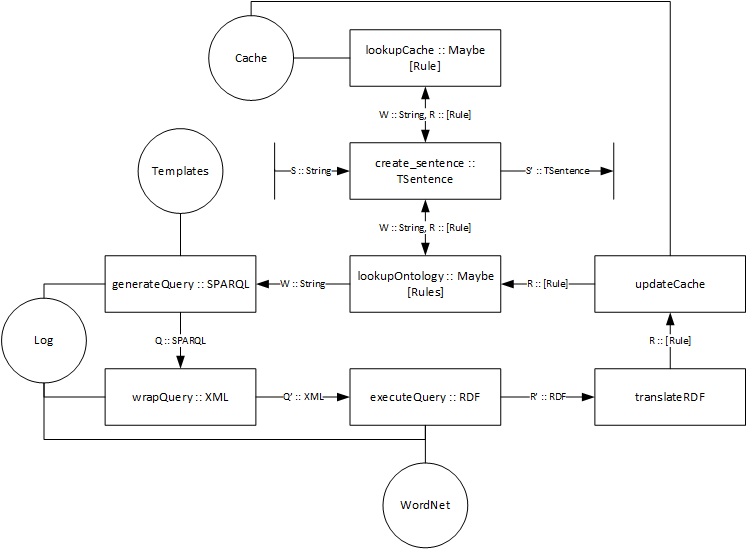
\includegraphics[scale=0.8]{images/typedstructure.png}
	\caption{\small Уточнённая структурная модель Модуля}
	\label{fig:typedstructure}
\end{figure} 

Приведённая модель опирается на принципы функционального программирования, то есть, разработку программ на основе их функциональной структуры и потоков данных, а не последовательности выполнения процедур (как в императивном программировании). Обозначения на рисунке \ref{fig:typedstructure}:

\begin{list}{\labelitemi}{\leftmargin=1.5cm}
	\item create_sentence --- точка входа, основная функция, принимающая на вход строку S и возвращающая размеченную строку S';
	\item lookupCache --- ищет в кэше правила по слову W, в соответствии с монадой Maybe, возвращает список правил R либо пустое значение;
	\item lookupOntology --- точка входа в подпроцесс поиска слова в онтологии, принимает на вход слово W, возвращает список правил R;
	\item generateQuery --- с помощью хранилища шаблонов на основе слова W генерирует SPARQL-запрос Q, описывая все действия в журнале Модуля;
	\item wrapQuery --- оборачивает запрос Q в форму Q', пригодную для передачи по сети;
	\item executeQuery --- отсылает запрос Q' на сервер онтологии, дожидается ответа, пишет результат в журнал;
	\item translateRDF --- транслирует полученный RDF-ответ R' в список правил (возможно, пустой) R;
	\item updateCache --- обновляет кэш, записывая туда соответствие списка правил R слову W, после чего завершает работу, возвращая полученный список в точку входа.
\end{list}

\subsection{Результаты и выводы по главе 3}

При проектировании Модуля были достигнуты следующие результаты:
\begin{list}{\labelitemi}{\leftmargin=1.5cm}
	\item сформулированы требования к функционированию, структуре и платформе проектируемой системы;
	\item структура прототипа разложена на программные функции верхнего уровня, уточнена схемой движения информации и типизирована;
	\item выполнено системно обоснованное техническое задание на разработку модуля взаимодействия парсера русского языка с онтологией (приложение А).
\end{list}

\textbf{Вывод}: полученной в результате проектирования информации достаточно для перехода к стадии инженерной реализации проекта.